\documentclass{myhw}
\usepackage{ctex}
\linespread{1.05}        % Palatino needs more leading (space between lines)
\usepackage{extarrows}
\usepackage{mathrsfs}
\usepackage{braket}
\usepackage{enumerate}
\usepackage{tikz}
\usepackage[ruled]{algorithm2e}
\usepackage{tikz-network}
\titleformat{\section}[runin]{\sffamily\bfseries}{}{}{}[]
\titleformat{\subsection}[runin]{\sffamily\bfseries}{}{}{}[]
\renewcommand{\exname}{Exercise }
\renewcommand{\subexcounter}{(\alph{homeworkSectionCounter})}
\newcommand{\id}{\text{Id}}
\newcommand{\tr}{\text{Tr}}
\newcommand{\rib}{\text{Rib}}

\title{Design and Analysis of Algorithms}

\begin{document}
\begin{center}
\noindent{\Large \heiti 2020年算法设计与分析 \textbf{Assignment-1}}

\vspace{0.5cm}

Due: OCT 19, 2020

\vspace{0.5cm}
\noindent {\large 郭宇航  202021080728}
\end{center}
\begin{homeworkProblem}
求解下列递归式的渐进解:
\[
\begin{split}
&(1)\quad f(n)=9f(n/6)+n\log n\\
&(2)\quad f(n)=2f(n-3)+n\\
&(3)\quad f(n)=4f(n/2)+n^2
\end{split}
\]

\end{homeworkProblem}
\begin{solution}
(1) 由于$f(n)=n\log n$,因为无法直接使用简单的master theorem求解。但是我们可以使用主定理对其进行分析。首先不难得到$a=9,b=6$. 那么$n^{\log_b a}=n^{\log_6 9}$, 同时$f(n)=n\log n$. 
\[
\frac{n^{\log_6 9}}{n\log n}=\frac{n^{(\log_6 9) -1}}{\log n}=\frac{n^{\log_6 \frac{3}{2}}}{\log n}
\]
由于分子是一个多项式时间复杂度,分母是一个对数时间复杂度,所以我们可以认为$f(n)$是要多项式地小于$n^{\log_b a}$的,也就是说我们能够找到一个$\epsilon >0$使得$f(n)=O(n^{\log_b (a-\epsilon)})$. 因此我们可以得到:
\[
T(n)=\Theta(n^{\log_6 9})
\]
\end{solution}
\begin{solution}
(2) 由于$f(n)=2f(n-3)+n$的形式不能够满足$b>1$的情况,因此这个问题无法使用master theorem处理。这里考虑使用递归树的方式处理,考虑这个递推关系式,对于原规模为$n$的问题,可以分解为两个规模为$n-3$的子问题,层层递归下去,我们不难发现这个递归树一共会有$n/3$层,同时每一层进行的运算为$n,n-3,n-6,\cdots$. 从而总运算数可以表示为一个等差数列的和:
\[
T(n)=\frac{n+1}{2}\times \frac{n}{3}=\frac{n^2+n}{6}
\]
从而问题的结果为:$T(n)=\Theta(n^2)$.
\end{solution}

\begin{solution}
(3) 这个问题可以直接使用master theorem进行求解:$a=4,b=2,c=2$.
得到$c=2=\log_b a=\log_2 4=2$.
因此这个问题的结果为:$T(n)=\Theta(n^2\log n)$.
\end{solution}
\begin{homeworkProblem}
将下列6个函数按照渐近增长率由低到高进行排序,要求写出判断依据。
\[
\begin{split}
&f_1(n)=\sqrt{n}+(\log n)^n,\quad f_2(n)=2^{\log n +\log \log n},\quad f_3(n)=\log\left(n^{100}\times 3^n\right)\\
& f_4(n)=n^{200}+3^{n},\quad f_5(n)=\log n^{100\log n},\quad f_6(n)100^n+n!\\
&(\text{各log函数的底数都为}2)
\end{split}
\]
\end{homeworkProblem}
\begin{solution}
首先对6个函数进行化简:
\begin{itemize}
\item $f_1(n)=\sqrt{n}+(\log n)^{100}$ 多项式时间
\item $f_2(n)=2^{\log n+\log \log n}=n\log n$.
\item $f_3(n)=\log (n^{100}\times 3^n)=100\log n+n\log 3$ 多项式时间
\item $f_4(n)=n^{200}+3^n$ 指数时间
\item $f_5(n)=\log n ^{100\log n}=100 \log n \log n$
\item $f_6(n)=100^n+n!$ 阶乘时间
\end{itemize}
经过化简之后可以很容易地得到关于这6个函数渐近增长率由低到高的排序:
\[
f_5(n)<f_1(n)<f_3(n)<f_2(n)<f_4(n)<f_6(n)
\]
\end{solution}
\begin{homeworkProblem}
平面上有$N\times M$个格子,每个格子中放着一定数量的苹果。从左上角的格子开始,每一步只能向下走或是向右走,每次走到一个格子上就把格子里的苹果收集起来,这样最终最多能收集到多少个苹果。设计算法求解上述问题,给出算法的伪代码描述即可。
\end{homeworkProblem}
\begin{solution}
使用简单的动态规划算法。假设定义平面为一个矩阵$W$,存储的是每个格子中对应的苹果数量。即$W[i][j]$表示的是第$i$行,第$j$列上的苹果的数量。另外我们再定义一个状态矩阵$S$用于存储每个位置上最多能够收集到的苹果数量。即$S[i][j]$表示再第$i$行,第$j$列上所能收集到的最多的苹果数量。由于题中要求从左上角的格子出发向下或者向右,因此在$(i,j)$位置上,可能获得的最多的苹果数量要么是来自左边的格子最大苹果数量加上当前格子的苹果数量,要么就是来自上面的格子最大的苹果数量加上当前格子的苹果数量。根据这个性质我们不难写出状态转移方程:$S[i][j]=W[i][j]+\max\{S[i][j-1],S[i-1][j]\}$.算法的时间复杂度为:$O(NM)$.\\
下面给出伪代码:\\
\begin{algorithm}[H]
\caption{最多苹果数量DP算法}
\LinesNumbered
\KwIn{$W[][]$, $N$, $M$}
\KwOut{$S[][]$}
\textbf{Initialize} State Matrix $S[N+2][M+2]$;\;
\For{$i = 1$ \textbf{To} $N$}{
  \For{$j =1$ \textbf{To} $M$}{
	  $S[i][j] = W[i][j] + \max \{S[i][j-1],S[i-1][j]\}$;
  }
}
\
\Return $S[N][M]$ 
\end{algorithm}
\end{solution}
\begin{homeworkProblem}
计算下图中从$S$到$T$的最大流,并给出最小割。
\begin{center}
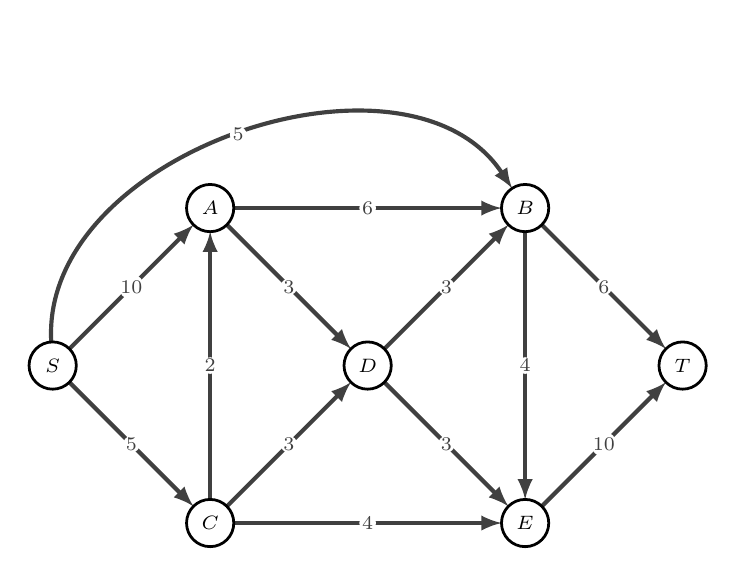
\begin{tikzpicture}
\Vertex[x=0,y=2,color=white,label=$S$]{S}
\Vertex[x=2,y=0,color=white,label=$C$]{C}
\Vertex[x=2,y=4,color=white,label=$A$]{A}
\Vertex[x=4,y=2,color=white,label=$D$]{D}
\Vertex[x=6,y=0,color=white,label=$E$]{E}
\Vertex[x=6,y=4,color=white,label=$B$]{B}
\Vertex[x=8,y=2,color=white,label=$T$]{T}
\Edge[label=$10$,Direct=True](S)(A)
\Edge[label=$5$,Direct=True](S)(C)
\Edge[label=$2$,Direct=True](C)(A)
\Edge[label=$4$,Direct=True](C)(E)
\Edge[label=$3$,Direct=True](C)(D)
\Edge[label=$3$,Direct=True](A)(D)
\Edge[label=$6$,Direct=True](A)(B)
\Edge[label=$3$,Direct=True](D)(B)
\Edge[label=$3$,Direct=True](D)(E)
\Edge[label=$4$,Direct=True](B)(E)
\Edge[label=$6$,Direct=True](B)(T)
\Edge[label=$10$,Direct=True](E)(T)
\Edge[bend=75,label=$5$,Direct=True](S)(B)
\end{tikzpicture}
\end{center}
\end{homeworkProblem}
\begin{solution}
首先使用贪心算法得到一个流$f_0$:$f_0=16$.贪心结果表示如下:
\begin{center}
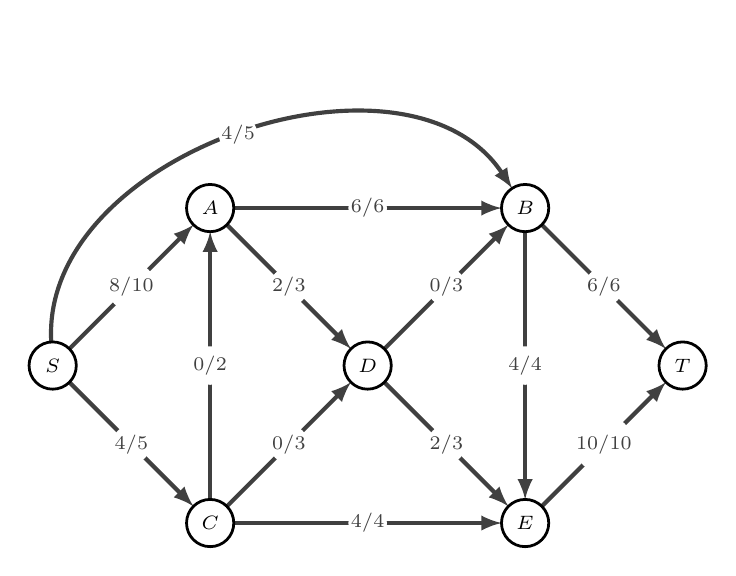
\begin{tikzpicture}
\Vertex[x=0,y=2,color=white,label=$S$]{S}
\Vertex[x=2,y=0,color=white,label=$C$]{C}
\Vertex[x=2,y=4,color=white,label=$A$]{A}
\Vertex[x=4,y=2,color=white,label=$D$]{D}
\Vertex[x=6,y=0,color=white,label=$E$]{E}
\Vertex[x=6,y=4,color=white,label=$B$]{B}
\Vertex[x=8,y=2,color=white,label=$T$]{T}
\Edge[label=$8/10$,Direct=True](S)(A)
\Edge[label=$4/5$,Direct=True](S)(C)
\Edge[label=$0/2$,Direct=True](C)(A)
\Edge[label=$4/4$,Direct=True](C)(E)
\Edge[label=$0/3$,Direct=True](C)(D)
\Edge[label=$2/3$,Direct=True](A)(D)
\Edge[label=$6/6$,Direct=True](A)(B)
\Edge[label=$0/3$,Direct=True](D)(B)
\Edge[label=$2/3$,Direct=True](D)(E)
\Edge[label=$4/4$,Direct=True](B)(E)
\Edge[label=$6/6$,Direct=True](B)(T)
\Edge[label=$10/10$,Direct=True](E)(T)
\Edge[bend=75,label=$4/5$,Direct=True](S)(B)
\end{tikzpicture}
\end{center}
在使用贪心算法得到一个解之后,画出现有网络的残余网络,寻找增广路径:
\begin{center}
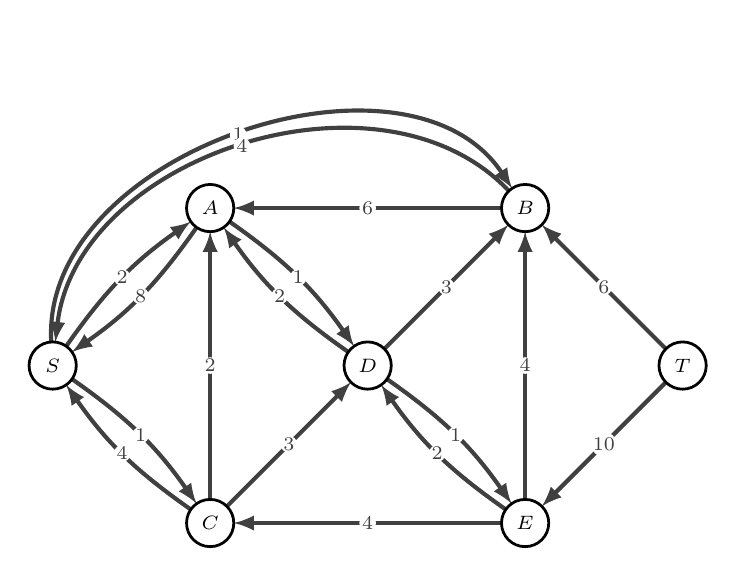
\begin{tikzpicture}
\Vertex[x=0,y=2,color=white,label=$S$]{S}
\Vertex[x=2,y=0,color=white,label=$C$]{C}
\Vertex[x=2,y=4,color=white,label=$A$]{A}
\Vertex[x=4,y=2,color=white,label=$D$]{D}
\Vertex[x=6,y=0,color=white,label=$E$]{E}
\Vertex[x=6,y=4,color=white,label=$B$]{B}
\Vertex[x=8,y=2,color=white,label=$T$]{T}
\Edge[bend=10,label=$2$,Direct=True](S)(A)
\Edge[bend=10,label=$8$,Direct=True](A)(S)
\Edge[bend=10,label=$1$,Direct=True](S)(C)
\Edge[bend=10,label=$4$,Direct=True](C)(S)
\Edge[bend=0,label=$2$,Direct=True](C)(A)
\Edge[bend=0,label=$4$,Direct=True](E)(C)
\Edge[bend=0,label=$3$,Direct=True](C)(D)
\Edge[bend=10,label=$1$,Direct=True](A)(D)
\Edge[bend=10,label=$2$,Direct=True](D)(A)
\Edge[bend=0,label=$6$,Direct=True](B)(A)
\Edge[bend=0,label=$3$,Direct=True](D)(B)
\Edge[bend=10,label=$1$,Direct=True](D)(E)
\Edge[bend=10,label=$2$,Direct=True](E)(D)
\Edge[bend=0,label=$4$,Direct=True](E)(B)
\Edge[bend=0,label=$6$,Direct=True](T)(B)
\Edge[bend=0,label=$10$,Direct=True](T)(E)
\Edge[bend=75,label=$1$,Direct=True](S)(B)
\Edge[bend=-65,label=$4$,Direct=True](B)(S)
\end{tikzpicture}
\end{center}
在画出的残余网络中我们发现无法找到一个增广路径,因此这个网络的最大流为$f=16$.\\
根据最大流最小割定理为:最小割$c=16$, 点集$A=\{S,A,B,C,D,E\}$, 点集$B=\{T\}$. 在最小割中的边为:$BT,ET$.
\begin{center}
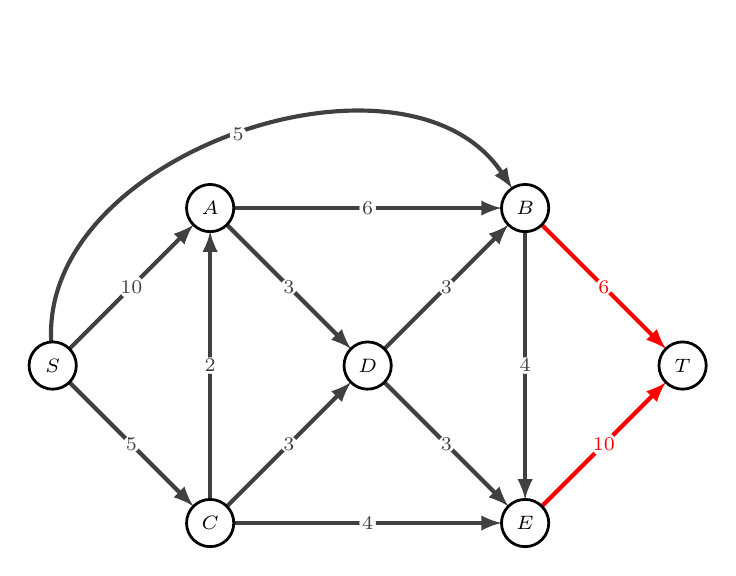
\begin{tikzpicture}
\Vertex[x=0,y=2,color=white,label=$S$]{S}
\Vertex[x=2,y=0,color=white,label=$C$]{C}
\Vertex[x=2,y=4,color=white,label=$A$]{A}
\Vertex[x=4,y=2,color=white,label=$D$]{D}
\Vertex[x=6,y=0,color=white,label=$E$]{E}
\Vertex[x=6,y=4,color=white,label=$B$]{B}
\Vertex[x=8,y=2,color=white,label=$T$]{T}
\Edge[label=$10$,Direct=True](S)(A)
\Edge[label=$5$,Direct=True](S)(C)
\Edge[label=$2$,Direct=True](C)(A)
\Edge[label=$4$,Direct=True](C)(E)
\Edge[label=$3$,Direct=True](C)(D)
\Edge[label=$3$,Direct=True](A)(D)
\Edge[label=$6$,Direct=True](A)(B)
\Edge[label=$3$,Direct=True](D)(B)
\Edge[label=$3$,Direct=True](D)(E)
\Edge[label=$4$,Direct=True](B)(E)
\Edge[label=$6$,Direct=True,color=red](B)(T)
\Edge[label=$10$,Direct=True,color=red](E)(T)
\Edge[bend=75,label=$5$,Direct=True](S)(B)
\end{tikzpicture}
\end{center}
\end{solution}
\end{document}
